%%%%%%%%%%%%%%%%%%%%%%%%%%%%%%%%%%%%%%%%
%%     Title and ToC
%%%%%%%%%%%%%%%%%%%%%%%%%%%%%%%%%%%%%%%%
% titlepage
\frame{
  \maketitle
}

\setcounter{footnote}{0}
\begin{frame}[noframenumbering]
\frametitle{The pbdR Core Team}
\begin{minipage}{3.6cm}
Wei-Chen Chen$^1$ \\
George Ostrouchov$^{1,2}$ \\
Pragneshkumar Patel$^2$ \\
Drew Schmidt$^2$ \\[2ex]
\end{minipage}
\begin{minipage}{7cm}
  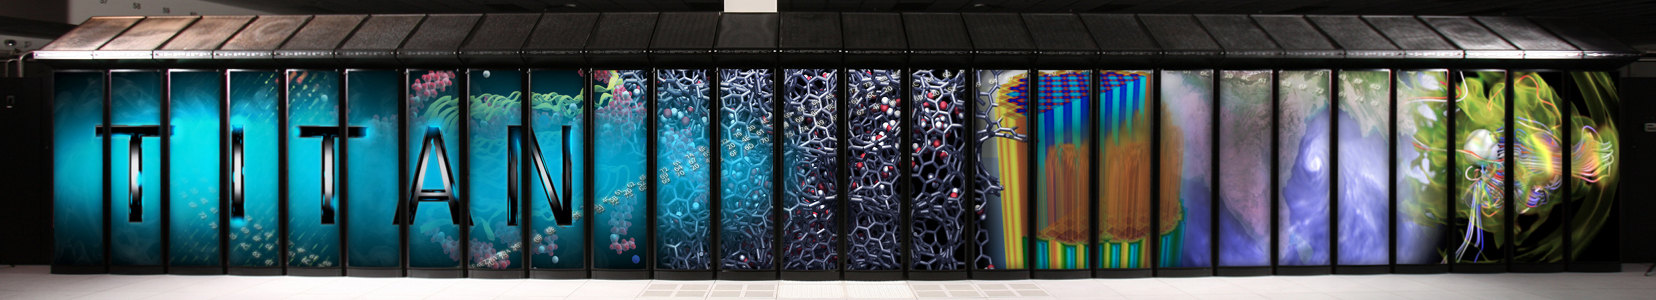
\includegraphics[width=7cm]{../common/pics/titan1wide} \\
  \tiny\bf 299,008 Cores and 18,688 GPUs in 18,688 Nodes with
  762 TB Memory \\
\end{minipage}

\vspace{-1.5em}
\begin{block}{Support}\tiny
  This work used resources of the \textcolor{blue}{Oak Ridge
    Leadership Computing Facility} at the Oak Ridge National
  Laboratory, which is supported by the Office of Science of the
  U.S. Department of Energy under Contract No. DE-AC05-00OR22725. This
  work also used resources of \textcolor{blue}{National Institute for
    Computational Sciences} at the University of Tennessee, Knoxville,
  which is supported by the Office of Cyberinfrastructure of the
  U.S. National Science Foundation under Award
  No. ARRA-NSF-OCI-0906324 for NICS-RDAV center. This work used
  resources of the Newton HPC Program at the University of Tennessee,
  Knoxville.

  \tiny \vspace{1em}$^1$Oak Ridge National Laboratory. Supported in
  part by the project ``Visual Data Exploration and Analysis of
  Ultra-large Climate Data'' funded by U.S. DOE Office of Science
  under Contract No. DE-AC05-00OR22725.

  \vspace{1em}$^2$University of Tennessee. Supported in part by the
  project ``NICS Remote Data Analysis and Visualization Center''
  funded by the Office of Cyberinfrastructure of the U.S. National
  Science Foundation under Award No. ARRA-NSF-OCI-0906324 for
  NICS-RDAV center.
\end{block}
\end{frame}

\begin{frame}[noframenumbering,shrink]
\frametitle{Contents}
\small
\tableofcontents[hideallsubsections]
\end{frame}

\setcounter{framenumber}{0}
